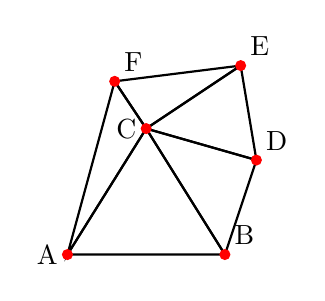
\begin{tikzpicture}
    % Punkte
    \coordinate (A) at (0,0);
    \coordinate (B) at (2,0);
    \coordinate (C) at (1,1.6);
    \coordinate (D) at (2.4,1.2);
    \coordinate (E) at (2.2,2.4);
    \coordinate (F) at (0.6,2.2);
    
    % Triangles (aus Delaunay-Triangulation)
    \draw[thick] (A) -- (B) -- (C) -- cycle;
    \draw[thick] (B) -- (C) -- (D) -- cycle;
    \draw[thick] (C) -- (D) -- (E) -- cycle;
    \draw[thick] (C) -- (E) -- (F) -- cycle;
    \draw[thick] (A) -- (C) -- (F) -- cycle;
    
    % Punkte markieren
    \foreach \p/\name in {A/A, B/B, C/C, D/D, E/E, F/F} 
    {
        \fill[red] (\p) circle (2pt);
    }    
    
    \node[left] at (A) {A};
    \node[above right] at (B) {B};
    \node[left] at (C) {C};
    \node[above right] at (D) {D};
    \node[above right] at (E) {E};
    \node[above right] at (F) {F};
\end{tikzpicture}
